\section{System with sequential composition}
    We model a first system with two sequentially composed component. We choose two model the two components as M/M/1/K queues. 
   
   \paragraph{Why M/M/1/K queues?} An average component in a distributed system can be modeled as an M/M/1/K, due to the exponential inter-arrival rate of messages $\lambda$, the exponential distribution of the execution delay $\mu$, the buffer size of messages $K$ of a component and the failure rate $f$. \cite{dq-tut}
    
    Let us first provide a refresher about M/M/1/K queues:
    \begin{itemize}
        \item $\lambda$: The arrival rate.
        \item s: The service time, is the time it takes to serve a message.
        \item $\mu$: The service \textbf{rate} and E[s] = $\dfrac{1}{\mu}$
        \item Offered load: $\rho = \dfrac{\lambda}{\mu}$
    \end{itemize}

    We will control $\lambda$ to show its effects on the offered load. The offered load can tell much about the system:
    \begin{itemize}
        \item At low load ($\rho < 0.8$) the failure will tend to 0, the system is behaving correctly and the $\Delta$Q will show that, the delay will tend to 1.
        \item Once $\rho$ is approaching high load ($\rho > 0.8$) we can observe the failure increasing quickly, but we can observe the system starting to get bad after $\rho > 0.5$! \cite{dq-tut}
    \end{itemize}
    
    \subsection{System composition}
    The system has two components \texttt{worker\_1}, \texttt{worker\_2}. Each individual component is made of a buffer queue of size $K = 1000$ and a worker process.
    
    The system sends $n$ messages per second following a Poisson distribution to \texttt{worker\_1}'s queue, the queue then reduces its available buffer size.
    
    The buffer notifies its worker, which then does $N$ loops, which are defined upon start, of fictional work. The worker then passes a message to \texttt{worker\_2}'s queue, which has another queue of same size, who passes the message to \texttt{worker\_2}'s worker, which does the same amount of loops. When a worker completes its work, it notifies the queue, freeing one "message" from its buffer size and allowing the next message to be executed.
    
    If the queue's buffer is overloaded, it will drop the incoming message and consider the execution a failure.
    
    A probe "$probe$" is defined, which observes the execution from when the message is sent to \texttt{worker\_1} up until \texttt{worker\_2} is done.
    \begin{figure}[H]
        \begin{center}
            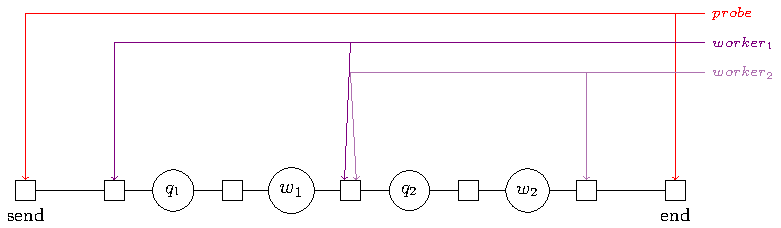
\includegraphics[scale=1.2, width=\textwidth]{tikz/mm1k.pdf} 
        \end{center}
        \caption{Outcome diagram of the M/M/1/K queue with the colored lines representing the probes that were inserted.}
        \label{fig:mm1k}
    \end{figure}

    \subsection{Determining parameters dynamically}
        We stated previously that determining parameters is something that must be done with an underlying knowledge of the system. The oscilloscope can provide knowledge of the system, here is an example of worker\_1 and worker\_2 as observed in the oscilloscope.

        Imagine the engineer supposes the workers executions should a maximum of 4 ms to complete, but doesn't actually know how long the executions should take. The engineer, after having set the required parameters observes in the following graph in the oscilloscope \cref{fig:w1w2}.

    The oscilloscope shows the engineer that their assumptions do not correspond to the actual system $\Delta$Q, the user can then modify the parameters to observe the actual system's behaviour. By setting $dMax$ to 8 ms, they can observe the worker's $\Delta$Qs failure approaching 0.

\begin{figure}[H]
            \centering
            \begin{subfigure}{.5\textwidth}
                \centering
                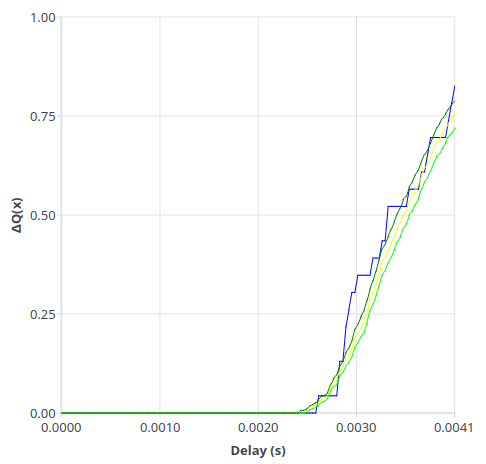
\includegraphics[width=0.98\textwidth]{img/overload_2/worker_1.png}
                \label{fig:w1w2}
                \subcaption{worker\_1 $\Delta$Q with confidence bounds plot with 4 ms $dMax$.}
            \end{subfigure}%
            \begin{subfigure}{.5\textwidth}
                \centering
                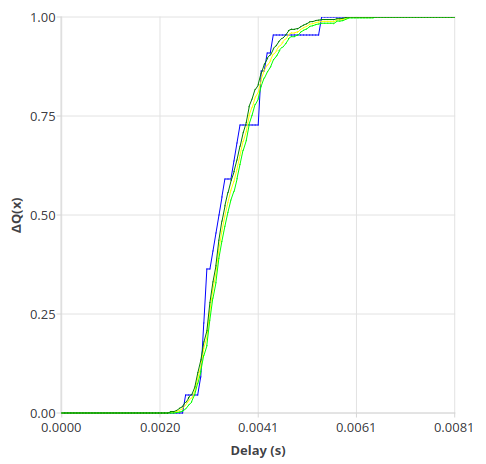
\includegraphics[width =0.98\textwidth]{img/overload_2/worker_1_8.png}
                \label{fig:sub2}
                \subcaption{worker\_1 $\Delta$Q wiht confidence bounds plot with 8 ms $dMax$} 
            \end{subfigure}
            \label{fig:w1w2hb}
            \end{figure}

    On the other hand, the engineer's assumption could have been what he truly expected from the system, in this case, the oscilloscope tells him that the system is not behaving as expected. 

    \subsubsection{Low Load} 
    Let's first observe the system at low load, we will send 50 messages per second to observe the system under test to get key properties.

        \begin{figure}[H]
            \centering
            \begin{subfigure}{.5\textwidth}
                \centering
                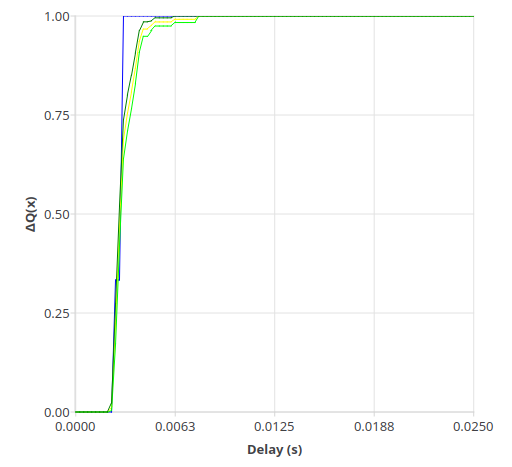
\includegraphics[width=0.98\textwidth]{img/overload_2/50_worker.png}
                \label{fig:norm_ex_1}
            \end{subfigure}%
            \begin{subfigure}{.5\textwidth}
                \centering
                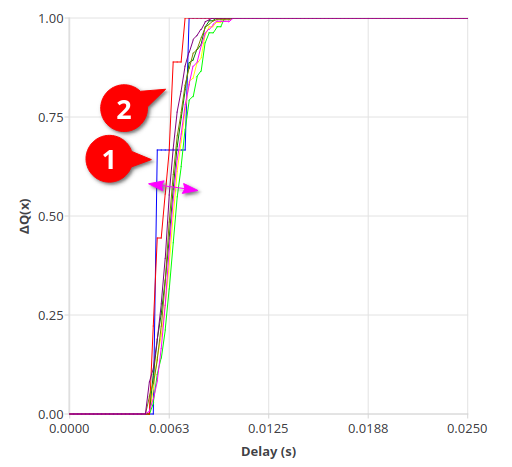
\includegraphics[width =0.98\textwidth]{img/overload_2/50_probe2.png}
                \label{fig:norm_ex_2}
            \end{subfigure}
            \label{fig:norm_ex}
            \caption{Left: worker\_1 $\Delta$Q, in blue, the observed $\Delta$Q, in green, the confidence bounds. Right: probe $\Delta$Q, in blue, the observed $\Delta$Q, in red the calculated $\Delta$Q. In magenta, the two $\Delta$Qs confidence bounds overlapping.}
        \end{figure}
    
    We first observe the worker's $\Delta$Q, we can observe that the average execution takes $\approx$ 30ms. We then have $\mu_{worker} = \dfrac{1}{0.0033} \approx 300$ req/s. Thus $\rho = \dfrac{50}{322} = 0.16$, we are in nice grounds!

    At low load, we can observe in the oscilloscope the probe \textbf{observed $\Delta$Q} and \textbf{calculated $\Delta$Q} confidence bounds overlap. 

\subsubsection{Early signs of overload}
    
    We can see how even at load = 0.5 the system is starting to show bad behaviour. Let us observe what happens when $\lambda = 150 \rightarrow \rho = 0.5$.

    \begin{figure}[H]
        \begin{center}
        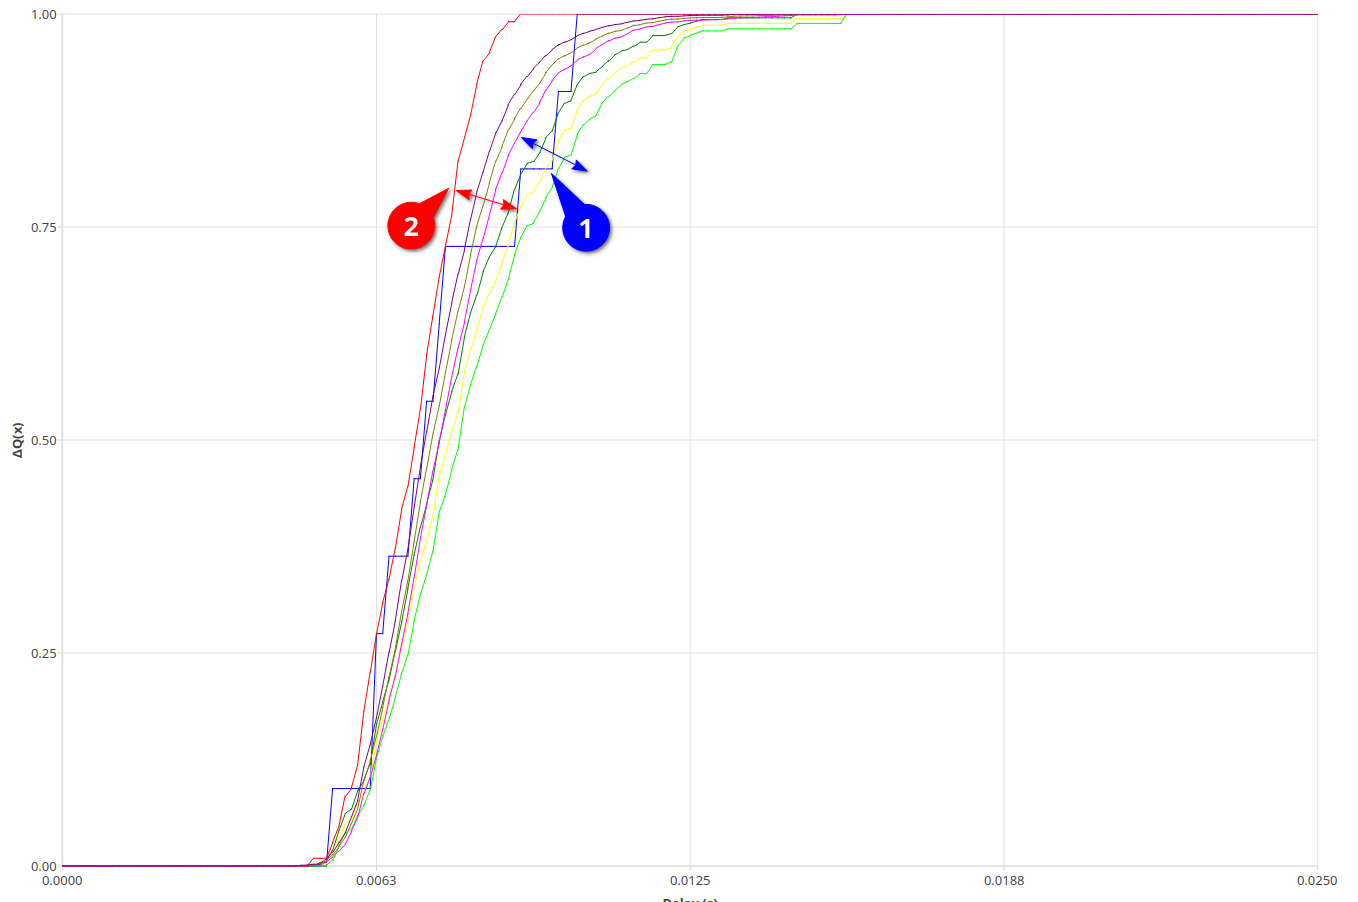
\includegraphics[scale = 0.3]{img/overload_2/150_probe2.png}
        \end{center}
            \caption{probe $\Delta$Qs, in blue (1), the observed $\Delta$Q, in red (2) the calculated $\Delta$Q. Arrow, above, blue: Observed $\Delta$Q confidence bounds. Arrow, below, red: Calculated $\Delta$Q confidence bounds.}%
        \label{fig:early_ov}
    \end{figure}
    
    \begin{figure}[H]
        \begin{center}
                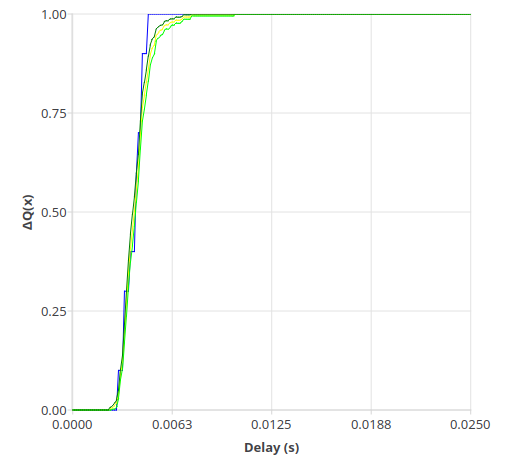
\includegraphics[scale=0.6]{img/overload_2/150_worker.png}
        \end{center}
            \caption{worker\_1 $\Delta$Q (blue) and its confidence bounds}.
        \label{fig:op}
    \end{figure}
    

    Recall \ref{fig:cdf_indep}, we can start to observe early signs of dependency! At load 0.5 the calculated $\Delta$Q is deviating from the observed one. This is a sign that the performance is degrading. Worker\_1 is slowing down, but we nevertheless do not observe failures in probe's $\Delta$Qs.

\subsubsection{High load}
    Performance at 0.5 offered load are already remarkable, the $\Delta$Qs are shifting.    We can go even further and observe the system under high load situations. We set $\lambda = 200 \rightarrow \rho = 0.83$, just above the high load threshold.
    
       \begin{figure}[H]
            \centering
            \begin{subfigure}{.5\textwidth}
                \centering
                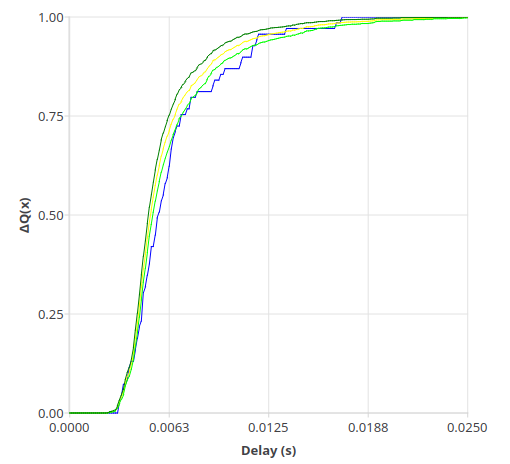
\includegraphics[width=0.98\textwidth]{img/overload_2/250_worker.png}
                \label{fig:high_load_1}
            \end{subfigure}%
            \begin{subfigure}{.5\textwidth}
                \centering
                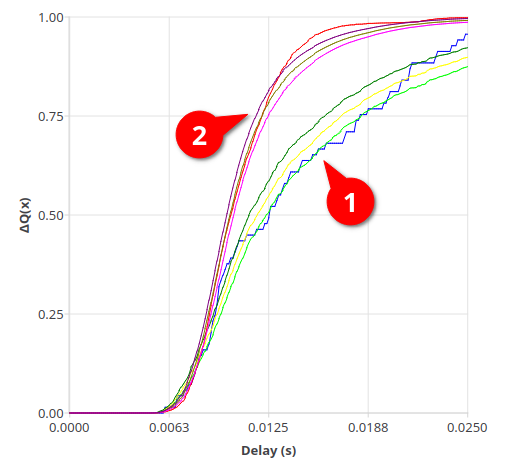
\includegraphics[width =0.98\textwidth]{img/overload_2/250_probe2.png}
                \label{fig:high_load_2}
            \end{subfigure}
            \label{fig:early_ov}
            \caption{Left: worker\_1 $\Delta$Q. Right: probe $\Delta$Q, in blue (1), the observed $\Delta$Q with its confidence bounds, in red (2) the calculated $\Delta$Q with its confidence bounds.}
        \end{figure}
    
    This is what we expected previously, and confirms what is expected by queueing theory, $\Delta$Q is capable of observing the basic observation requirements and capable of recognising dependency. While what is expected by the execution of the queue (observed $\Delta$Q) is a nice normally distributed CDF with little to no failure. What we can actually observe is a degraded performance in both workers and the probe observed execution.

    The workers CDF has completely degraded, with the average request taking almost double the time as under normal queueing conditions. 

    Further degradation can be observed by increasing $\lambda = {300, 350} \rightarrow \rho \ge 1$.

    \begin{figure}[H]
            \centering
            \begin{subfigure}{.5\textwidth}
                \centering
                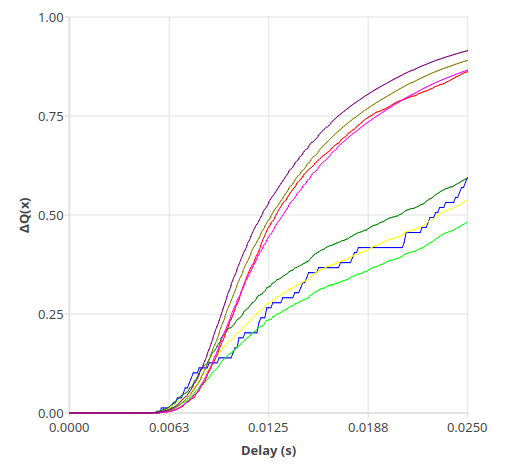
\includegraphics[width=0.98\textwidth]{img/overload_2/300_probe.png}
                \label{fig:high_load_1}
            \end{subfigure}%
            \begin{subfigure}{.5\textwidth}
                \centering
                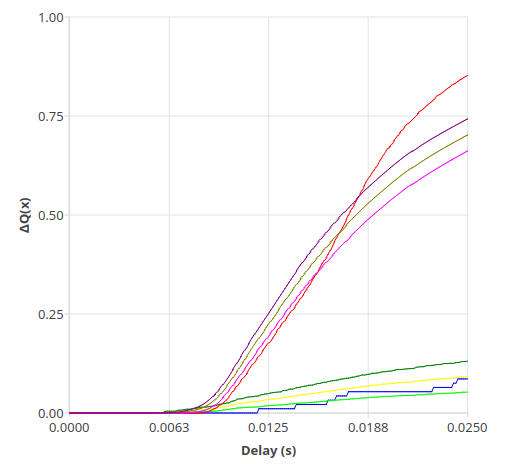
\includegraphics[width =0.98\textwidth]{img/overload_2/350_probe.png}
                \label{fig:high_load_2}
            \end{subfigure}
            \label{fig:early_ov}
            \caption{Left: probe $\Delta$Qs at $\lambda = 300$. Right: probe $\Delta$Qs at $\lambda = 350$}
        \end{figure}

    The system degrading clear, the $\Delta$Qs show how almost all messages are being dropped or take $> dMax$. Let us look at triggers and how they can be useful to diagnose such cases.
  
    \subsubsection{Triggers}
        By observing the system under test in high load cases, we can set the load trigger by setting the sampling window to 1 second and trigger when outcome instances $\gtrapprox 150$. We can also set a trigger based on observation of the running system.

        \paragraph{QTA trigger}
            By observing the system, we create a QTA for the probe with: 25\% = 0.0075 s, 50\% = 0.0125 s, 75\% = 0.015s and minimum intangible mass = 0.9.

            By setting the trigger to fire for $\Delta$Q$_{obs} < QTA$. We captured a handful of snapshots. Here, $\lambda = 150$.
        
        \begin{figure}[H]
            \centering
            \begin{subfigure}{.5\textwidth}
                \centering
                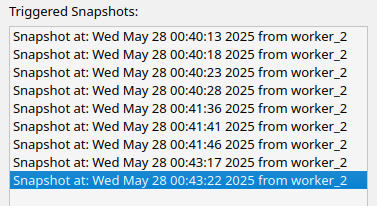
\includegraphics[width=0.98\textwidth]{img/overload_2/snapshots.png}
                \label{fig:high_load_1}
            \end{subfigure}%
            \begin{subfigure}{.5\textwidth}
                \centering
                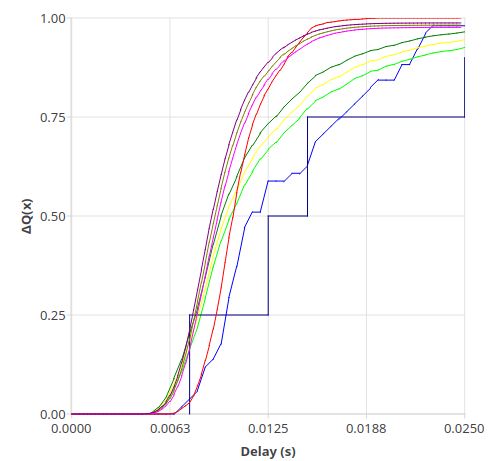
\includegraphics[width =0.98\textwidth]{img/overload_2/qta_fired.png}
                \label{fig:high_load_2}
            \end{subfigure}
            \label{fig:early_ov}
            \caption{Left: Fired triggers. Right: Sample QTA violation.} % 
        \end{figure}

    QTA triggers can help to detect overhead even before high load becomes evident!

        \paragraph{Instances trigger}
        By knowing the inner details of the system, setting a QTA on the number of instances can be useful. Here is an example of a fired trigger on the number of instances.

        Even though the QTA requirement isn't being violated, the number of instances fires a trigger, where the user can observe that the system is showing early signs of overload.
        \begin{figure}[H]
            \begin{center}
                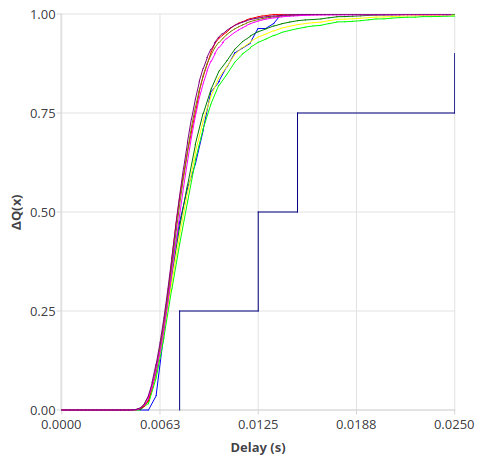
\includegraphics[scale=0.5]{img/overload_2/fired_sample.png}
            \end{center}
        \end{figure}
  
